	Following 
\appref{prop:chapters/11/11/1/pts},
\begin{align}
	\label{eq:chapters/11/11/1/10circPoints}
	\vec{x}_{1} = \myvec{4\\1},\ \vec{x}_{2} = \myvec{6\\5},\
	\vec{n} = \myvec{4 \\ 1},\  c= -16.
\end{align}
Substituting  in
	\eqref{eq:chapters/11/11/1/mat},
\begin{align}
	\myvec{
	        8 &  2 & 1\\
	       12 & 10 & 1\\
-4 & -1 & 0}
	\myvec{\vec{u}\\f} = 
	\myvec{16 \\ -61 \\ -17}
\end{align}
The augmented matrix is expressed as
\begin{align}
	\myvec{
	        8 &  2 & 1 & \vrule & -17\\
	       12 & 10 & 1 & \vrule & -61\\
-4 & -1 & 0 & \vrule & 16}
\end{align}
Performing a sequence of row operations to transform into an Echelon form
\begin{align*}
	\xleftrightarrow[R_2\rightarrow R_2+3R_1]{{R_3\rightarrow R_3+2R_1}}
	\myvec{-4 & -1 & 0 & \vrule & 16\\
	        0 &  7 & 1 & \vrule & -13\\
	        0 &  0 & 1 & \vrule & 15}
	\xleftrightarrow[]{{R_2\rightarrow R_2-R_3}}
	\myvec{-4 & -1 & 0 & \vrule & 16\\
	        0 &  7 & 0 & \vrule & -28\\
	        0 &  0 & 1 & \vrule & 15}\\
	\xleftrightarrow[]{{R_2\rightarrow \frac{R_2}{7},R_1\rightarrow \frac{-R_1}{4}}}
	\myvec{ 1 & \frac{1}{4} & 0 & \vrule & -4\\
	        0 &  1 & 0 & \vrule & -4\\
	        0 &  0 & 1 & \vrule & 15}
	\label{eq:chapters/11/11/1/10solution}	
	\xleftrightarrow[]{{R_1\rightarrow R_1-\frac{1}{4}R_2}}
	\myvec{ 1 &  0 & 0 & \vrule & -3\\
	        0 &  1 & 0 & \vrule & -4\\
	        0 &  0 & 1 & \vrule & 15}
\end{align*}
So, from \eqref{eq:chapters/11/11/1/10solution}
\begin{align}
	\vec{u} = -\myvec{3\\4},\
	f = 15.
\end{align}
See \figref{fig:chapters/11/11/1/10Fig1}.
\begin{figure}[H]
	\begin{center} 
	    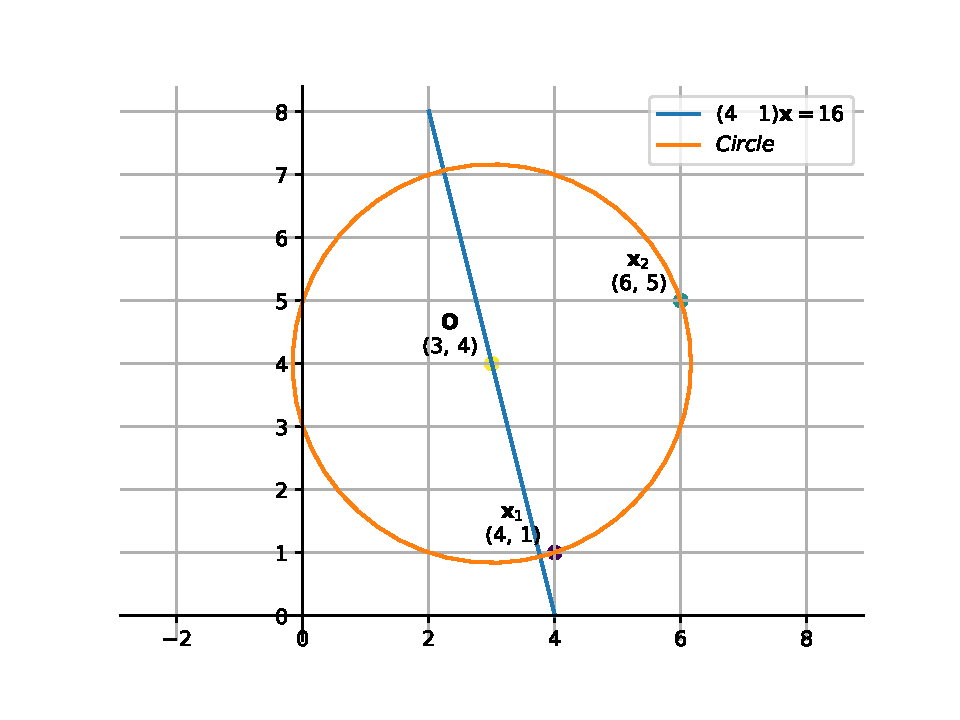
\includegraphics[width=0.75\columnwidth]{chapters/11/11/1/10/figs/fig.pdf}
	\end{center}
\caption{}
\label{fig:chapters/11/11/1/10Fig1}
\end{figure}





